\documentclass[conference,a4paper]{IEEEtran}
\usepackage[T1]{fontenc}
\usepackage[utf8]{inputenc}
\usepackage{amsmath,amssymb,graphicx,booktabs,array,microtype}
\usepackage[authoryear,round]{natbib}
\usepackage{xcolor}
\usepackage{ragged2e}
\usepackage{listings}
\usepackage[justification=raggedright,singlelinecheck=false,font=small]{caption}
\lstset{basicstyle=\ttfamily\scriptsize,backgroundcolor=\color{white},keywordstyle=\color{black},commentstyle=\color{black},stringstyle=\color{black},breaklines=true,breakatwhitespace=false,columns=fullflexible,keepspaces=true,showstringspaces=false,frame=single,rulecolor=\color{black!25},numbers=left,numberstyle=\tiny\color{black},numbersep=5pt,xleftmargin=1em}
\renewenvironment{abstract}{\par\noindent\textbf{Abstract}\par\smallskip\normalfont\normalsize\RaggedRight}{\par\medskip}
\renewenvironment{IEEEkeywords}{\par\noindent\textbf{Keywords: }\normalfont\normalsize\RaggedRight}{\par\medskip}
\usepackage{titlesec}
\titleformat{\section}{\normalfont\large\bfseries\raggedright}{\thesection}{1em}{}
\titleformat{\subsection}{\normalfont\normalsize\bfseries\raggedright}{\thesubsection}{1em}{}
\usepackage{xurl}
\usepackage[colorlinks=true,urlcolor=blue!55!black,citecolor=blue!55!black,linkcolor=blue!55!black]{hyperref}
\setlength{\emergencystretch}{2em}
\newcommand{\fig}[3]{\begin{figure}[t]\centering\includegraphics[width=\columnwidth]{images/#1.pdf}\caption{#2}\label{#3}\end{figure}}
\newcommand{\widefig}[3]{\begin{figure*}[t]\centering\includegraphics[width=.95\textwidth]{images/#1.pdf}\caption{#2}\label{#3}\end{figure*}}
\title{Machine Learning Approach for Forest Fire Risk Prediction in Nepal}
\author{\IEEEauthorblockN{Krijal Shrestha}\IEEEauthorblockA{Coventry ID: 11495103\\STW7072CEM Machine Learning\\Softwarica College of IT and E-commerce, Coventry University}}
\begin{document}
\makeatletter
\renewcommand{\@maketitle}{%
\newpage\null\vskip 1em%
{\raggedright\LARGE\bfseries\@title\par}%
\vskip 1em%
{\raggedright\normalsize Krijal Shrestha\\
Coventry ID: 11495103\\
STW7072CEM Machine Learning\\
Softwarica College of IT and E-commerce, Coventry University\par}%
\vskip 1.5em}
\makeatother
\maketitle
\RaggedRight
\begin{abstract}
This study compares Logistic Regression, Linear Support Vector Machine, Random Forest and Gradient Boosting for next-day forest-fire detection in Nepal. Fire records distributed by ICIMOD are combined with preceding daily weather, forest cover and terrain information. Data preparation includes checking dates, removing repeated detections, defining forest locations and constructing weather summaries using only earlier days. Models are trained on earlier years and evaluated on later observations. The comparison examines how well each method identifies recorded fire days while accounting for the large number of days without a detection. Model rankings differ between validation and testing, and adding weather improves the ranking of recorded fire days. The findings apply to the analysed forest-grid sample. Uncertain absence labels, limited observation years and prior exploratory use of some test records restrict wider conclusions.
\end{abstract}
\begin{IEEEkeywords}
Nepal, ICIMOD, forest fire, support vector machine, gradient boosting, imbalanced classification, temporal evaluation
\end{IEEEkeywords}

\section{Introduction}
Forest-fire prediction presents a practical machine-learning problem in which the most easily reported metric can conflict with the purpose of the application. A classifier can label almost every location-day as having no fire and obtain impressive accuracy when detections are rare. Such a model may offer little help in identifying the exceptional days that require attention. For a Nepal-focused study, evaluating this conflict is as important as fitting a technically sophisticated algorithm. The central question is therefore how different classifiers perform under the same data preparation and chronological evaluation, and what their apparent accuracy means for recorded fire detection.

The study uses fire records collected for Nepal. The International Centre for Integrated Mountain Development (ICIMOD) distributes MODIS-based active-fire incident locations for Nepal through its Regional Database System \citep{icimodfire}. ICIMOD is an intergovernmental knowledge organisation headquartered in Kathmandu, serving countries of the Hindu Kush Himalaya \citep{icimodabout}. Its regional role and location in Nepal make it an appropriate institutional source for this research, while the underlying observations remain satellite measurements. These distinctions matter: the records are neither locally installed weather-station readings nor a complete field census of every forest fire.

The submitted proposal named Logistic Regression, Random Forest and Gradient Boosting. This study retains those models and adds a Linear Support Vector Machine (SVM), which offers a margin-based comparison with the probability-based linear classifier and tree ensembles. All four methods use the same features and chronological partitions, so differences in their results can be interpreted against a common experimental design. The comparison focuses on methods suited to a binary, imbalanced classification task.

\subsection{Aim}
The aim is to compare machine-learning models for predicting next-day recorded forest-fire detections in Nepal using fire, weather and geographic data.

\subsection{Next-Day Forest-Fire Detection}
The model predicts whether a forest-containing grid cell will have at least one recorded active-fire detection on the next day. For example, to predict a detection on 15 April, the weather summaries end on 14 April. The output is a score for that cell and target date; a threshold chosen using the validation data converts the score into a detection or no-detection prediction. A recorded detection is coded as 1, and a day with no retained detection is coded as 0.

This definition gives a specific meaning to forest-fire risk in this paper. Satellite records provide evidence of detected heat, while a missing record does not prove that no fire occurred. The analysis therefore measures prediction of recorded detections. Historical reanalysis weather is used to test the method on past dates, so the results describe a retrospective experiment within the analysed grid sample.
\section{Related Research and Research Gap}
\subsection{Three foundation studies}
\citet{dhakal} compare fuzzy analytical hierarchy process, Random Forest and boosted regression trees for susceptibility mapping in Nepal's Chure Tarai Madhesh Landscape. They report Random Forest AUC of 0.95 and overall accuracy of 0.91. The study supports combining environmental factors and comparing different modelling approaches. Its landscape-specific susceptibility target does not directly establish performance for daily prediction at later dates. The gap addressed here is therefore an evaluation mismatch: the present study constructs grid-day labels and separates earlier training years from later evaluation years. This is an extension in task definition, not a claim that their study was incorrectly designed. The present study addresses a different question and its conclusions are bounded by the analysed grid-cell sample.

\citet{dahal} investigate Nepal's forest-fire susceptibility at sub-decadal scales using Random Forest and relate susceptibility to carbon stocks and biodiversity. Their national perspective demonstrates why fire analysis can matter beyond the location of individual detections. However, their multi-year spatial analysis does not answer which of several classifiers best discriminates daily recorded events under a common temporal split. This project responds through an explicit four-model comparison and lagged daily predictors. It does not reproduce their carbon or biodiversity assessments: those outcomes require additional labels and assumptions. The limitation identified here concerns transfer of evidence to this coursework's daily classification question, rather than a general deficiency of the original research.

\citet{sarkar} compare boosted regression trees, Random Forest, SVM, classification and regression trees, multivariate adaptive regression splines and an ensemble for forest-fire susceptibility in Northeast India. Their study provides regional motivation for testing methods beyond Random Forest and shows that model comparison is relevant to fire mapping. A limitation for the present application is geographic and task transfer: performance in Northeast India does not establish next-day detection performance in Nepal. The response is to fit the algorithms to Nepal-specific records and evaluate them chronologically. The SVM implemented here is explicitly linear; it is not presented as a replication of every configuration in that paper. Published susceptibility scores are not directly comparable with the results below.

\subsection{Research Gap and Proposed Solution}
Together, these studies motivate a narrower and testable research gap: for the particular ICIMOD incident export and weather integration used here, the relative behaviour of linear, margin-based and ensemble classifiers under chronological daily evaluation remains to be demonstrated. This is a dataset-specific experimental gap. It should not be inflated into a claim that daily fire forecasting has never been studied or that all previous research relies on Random Forest. The solution is an integrated experimental protocol that can be inspected and rerun, with model differences evaluated on identical observations.

There are three important distinctions between a susceptibility map and this target. First, a location may have a high long-term susceptibility while no detection occurs on a particular day. Second, a positive grid-day depends on satellite observation as well as the underlying fire process. Third, a classifier intended for later dates must not use weather or fire characteristics observed after the prediction origin. These distinctions determine the construction of the target, the choice of predictors and the split strategy. They also prevent inappropriate claims that a lower daily-classification metric disproves a higher metric from a spatial study.

Imbalanced evaluation provides the second methodological motivation. \citet{saito} explain why precision--recall analysis can reveal limitations that are less apparent in ROC analysis for imbalanced classification. This study accordingly reports accuracy, balanced accuracy, precision, recall, F1, average precision (AP), ROC-AUC and confusion counts. Balanced accuracy is emphasised because it gives equal weight to the two classes, while ordinary accuracy is retained to show the effect of class imbalance. AP summarises ranking over thresholds; F1 describes a particular threshold. Keeping these roles separate avoids using whichever metric happens to favour a preferred model.

\section{Study Data and Problem Definition}
\subsection{ICIMOD active-fire incidents}
The main file is \texttt{Active\_Fire\_Incidents\_in\_Nepal.csv}. It contains 13,781 rows and 25 columns, with acquisition dates from 1 February 2012 to 19 June 2016. Relevant fields include latitude, longitude, acquisition date and time, satellite identifier, confidence, brightness, fire radiative power, land-cover descriptors and administrative attributes. The ICIMOD catalogue describes MODIS-based Nepal incidents over February 2012--June 2016 and an overlay with land cover. It supplies a dataset DOI and a Creative Commons Attribution licence \citep{icimodfire}. The supplied CSV is retained unchanged; a checksum identifies the exact local input used in processing.

A single fire can produce several satellite detection rows. Clouds, satellite overpass times and gaps in the archive also mean that a day with no record may still have had a fire. The study therefore aggregates records into a grid-day target and calls it a ``recorded detection,'' not an independent ignition or confirmed fire absence.

The source has 3,149 rows in 2012, 1,999 in 2013, 2,386 in 2014, 489 in 2015 and 5,758 in 2016. The endpoint years are incomplete. The unusually small 2015 count is an audit concern, but the file alone cannot establish whether it reflects actual fire conditions, observation variation or missing records. The study does not fill that uncertainty with invented incidents. It retains the proposed validation year and discusses the resulting prevalence shift explicitly.

\subsection{Weather, land cover, terrain and boundary}
Weather is obtained from the Open-Meteo Historical Weather API with the model explicitly fixed to ERA5. The requested period is 1 January 2012--31 December 2016, supplying 1,827 daily dates at each location. Seven variables are downloaded: mean and maximum 2-m temperature, precipitation sum, mean and minimum relative humidity, and mean and maximum 10-m wind speed. Units are degrees Celsius, millimetres, percentage relative humidity and metres per second. Requests use Asia/Kathmandu daily aggregation, nearest-cell selection and disabled elevation adjustment. Open-Meteo is the access service; ERA5 is the underlying reanalysis \citep{openmeteo,hersbach}.

This differs from the proposal's ERA5-Land plan. The two products are not interchangeable descriptions, and the separately collected ERA5-Land months are not mixed into this experiment. The change provides a consistent daily dataset at the nominal 0.25-degree ERA5 spacing. It also means the paper does not claim to have derived humidity from downloaded dewpoint or wind speed from downloaded vector components: the service supplies those daily variables. Reanalysis provides spatially complete estimates, but it does not reproduce every local mountain microclimate or establish what would have been available operationally at midnight.

The forest mask comes from the 2011 layer of the Forest Research and Training Centre's national land-cover collection, distributed through ICIMOD \citep{frtc}. The original archive is \texttt{Land cover of Nepal 2011.zip}, containing \texttt{lc2011.tif}. Class 4 defines forest. The 2013--2016 archives were collected but are not used as predictors. A fixed pre-study baseline gives one consistent eligibility rule and avoids directly using later forest outcomes to explain earlier fires. It cannot represent forest gain or loss after 2011, and the retrospectively produced map should not be confused with a product demonstrably available in real time in 2011.

Elevation comes from the OpenTopography SRTM GL1 download \texttt{rasters\_SRTMGL1.tar.gz}. Its extracted raster is stored as \texttt{nepal\_SRTMGL1.tif}. The approximately 30-m terrain product represents the February 2000 SRTM acquisition, rather than annual terrain measurements for 2012--2016 \citep{srtm}. Elevation, slope and aspect summaries provide comparatively stable geographic context. No assumption is made that 30-m terrain resolution increases weather resolution to 30 m.

The country boundary is \texttt{geoBoundaries-NPL-ADM0.geojson}. Its supplied metadata identifies a 2019 boundary representation and an attribution licence. It restricts the forest mask and incident coordinates to the chosen Nepal polygon; it contains geometry and attributes, not environmental measurements. The boundary resource is documented by \citet{runfola}. Using a later administrative representation as a fixed mask is disclosed because it defines the study footprint rather than reconstructing historical administrative changes.

\subsection{Analytical grid and target}
The analytical grid consists of 218 forest-containing cell locations with complete daily weather histories. Each included location has 1,827 unique dates from 1 January 2012 through 31 December 2016, with finite values for all seven weather variables. The grid identifiers and source-file hashes are recorded in a manifest to make the experiment reproducible. Because the analysed cells are the locations with complete weather series in the available snapshot, the results describe this sample; geographic patterns should not be extrapolated to unrepresented parts of Nepal without further validation.

Let $g$ identify an eligible cell and $t$ a local calendar day. The target is
\begin{equation}
y_{g,t}=\mathbb{1}\!\left\{\text{at least one retained detection in }(g,t)\right\}.
\end{equation}
A zero means no retained recorded detection, not confirmed absence. The data retain all eligible grid-days, rather than selecting a matched sample of negative records. This preserves the observed class prevalence within the analysis footprint. A cell centre can lie outside the boundary while its cell intersects forest inside Nepal; eligibility is determined by forest pixels within the polygon, not by centre-point nationality.

\widefig{coverage_counts}{Study footprint and source counts. Colours show retained positive grid-days across the analysed forest-grid cells. Counts in the right panel are source rows before cleaning; 2012 and 2016 are partial years.}{fig:coverage}

\section{Data Preparation and Feature Engineering}
\subsection{Cleaning and integration}
The cleaning pipeline first checks acquisition dates and time fields. MODIS-style acquisition time is interpreted as UTC and converted to Asia/Kathmandu before daily aggregation. This convention remains an assumption for the supplied export, not a separately verified property of its processing history. All rows pass the implemented acquisition-time validity checks. Detections are sorted by confidence and deduplicated using latitude and longitude rounded to five decimal places, timestamp and satellite. This removes 224 repeated detection keys while retaining the highest-confidence version of each key. It does not merge an entire multi-pixel fire into one inferred incident.

One remaining point falls outside the supplied Nepal polygon. Sampling the 2011 forest raster removes a further 3,298 points that are not class 4 forest, leaving 10,258 forest detection rows before restriction to the available weather footprint and model dates. The source's original land-cover label is not substituted for this fixed-mask definition. This avoids applying inconsistent forest criteria to positive and negative examples. Different forest definitions could legitimately yield different labels, which is a sensitivity question rather than a reason to hide the choice.

Source administrative missing values are audited, but these columns are not predictors. No missing district name is imputed into an environmental feature. Included weather files are checked for duplicate dates, the exact expected date sequence, matching grid identifiers and finite numeric values. Rainfall is checked for nonnegative values and mean humidity for values within zero to one hundred. Prepared predictors have no missing values. Consequently, mean imputation or nearest-neighbour imputation is unnecessary for this snapshot and would add an unsupported processing step.

The model interval is 2 February 2012--18 June 2016. The first and last acquisition dates are excluded because the export does not establish full-day observation at either endpoint. This precaution does not establish complete monitoring on the remaining days. Fire points are assigned to the nearest nominal quarter-degree cell and joined to daily weather by cell identifier and local date. Multiple detections in one cell-day produce a single positive target. The final table contains 348,582 rows, including 4,344 positive grid-days, and no duplicated cell-date keys.

Terrain processing aligns elevation to the land-cover raster using bilinear resampling. Slope is derived from elevation gradients using approximate local metre distances, rather than treating a degree of latitude or longitude as a metre. Overlapping processing rows prevent artificial slope edges at block boundaries. Mean elevation, slope, northness and eastness are then calculated over forest pixels inside Nepal. Forest fraction is the count of forest pixels divided by classified pixels within the relevant clipped cell. These are spatial summaries; they do not imply that every forest pixel experiences the cell-average conditions.

\subsection{Predictors and mathematical construction}
Twenty-one predictors are used. Six are previous-day mean and maximum temperature, mean and minimum humidity, and mean and maximum wind speed. Three describe preceding precipitation totals over one, seven and thirty days. Two give preceding seven-day temperature and humidity means. One represents the preceding dry-day run. The remaining nine are latitude, longitude, forest fraction, mean elevation, mean slope, mean aspect northness and eastness, and sine/cosine seasonal terms.

For precipitation $P$, the rolling predictor is
\begin{equation}
R^{(k)}_{g,t}=\sum_{j=1}^{k}P_{g,t-j},\qquad k\in\{1,7,30\}.
\end{equation}
The analogous seven-day mean divides the sum of preceding temperature or humidity by seven. Every weather window ends at $t-1$. Independent checks recompute the previous-day temperature and thirty-day rainfall for every included location and compare them with the prepared table. This verifies that rolling features align with the target date rather than accidentally include the target day's weather.

A dry day is operationally defined here as precipitation below 1 mm. The dry-run feature counts consecutive preceding dry days and caps the count at thirty. This cap makes the lookback fully supported by the available January history, including for long dry spells that may have begun before downloading started. It is a pragmatic feature definition, not a measured fuel-moisture index. The cap and threshold are fixed before evaluation, rather than chosen for a favourable test score.

Day-of-year $d_t$ is represented cyclically:
\begin{equation}
S_t=\sin(2\pi d_t/365.25),\qquad C_t=\cos(2\pi d_t/365.25).
\end{equation}
This gives neighbouring calendar dates similar seasonal representations around the year boundary. Latitude and longitude encode broad spatial variation, while the forest and terrain features distinguish geographic context. Including location can improve later-time prediction at known cells but also encourages spatial dependence; the geographic diagnostic therefore tests a different and more difficult transfer setting.

Features measured as part of fire detection are excluded. Brightness, fire radiative power, acquisition hour, confidence and detection counts are unavailable in the same form for genuine negative examples and could reveal the target. A diagnostic flag indicating whether any national detection was recorded on a date is also excluded. Otherwise, the model could learn contemporaneous information from elsewhere in the target day. The feature list is written to a separate file and checked before fitting, making these exclusions reproducible.

\subsection{Distribution, scaling and imbalance}
Training-only distributions and Spearman correlations are examined before interpretation. Rainfall has a concentration of low values and a long upper tail; dry-day counts are bounded and accumulate at particular integer values. The predictors need not follow Gaussian distributions for the selected discriminative classifiers. Standardisation changes scale, not distributional shape. It is therefore inappropriate to claim that normalising these variables makes them normally distributed or that a normality test alone establishes suitability for classification.

For Logistic Regression and Linear SVM, each feature is transformed as
\begin{equation}
z_{ij}=(x_{ij}-\mu_j^{\mathrm{train}})/\sigma_j^{\mathrm{train}}.
\end{equation}
The mean and standard deviation are fitted only on training observations through a pipeline. Validation and test observations use those same values. This makes regularisation operate on comparable feature scales. Tree models use the original numeric predictors because their axis-aligned splits do not require the same scale equalisation. The correlation plot is diagnostic; no variable is removed because of its association with test performance.

The training imbalance is addressed through inverse-frequency class weights:
\begin{equation}
w_c=N/(2N_c),\qquad c\in\{0,1\},
\end{equation}
where $N_c$ counts training examples of class $c$. Random Forest uses balanced weights within each bootstrap sample. No negative downsampling or synthetic oversampling is performed. SMOTE creates interpolated minority examples \citep{chawla}, but unconstrained interpolation across geographic, seasonal and terrain predictors could create implausible environmental combinations here. Class weighting changes the fitting objective without inventing locations or observations. It does not correct missing positive labels or guarantee calibrated probabilities.

\widefig{distributions}{Training-only feature distributions. Precipitation is visibly asymmetric; a dry-day run is discrete and capped. Scaling is used for numerical comparability, not to impose normality.}{fig:distributions}
\fig{correlation}{Selected training-only Spearman correlations. Red and blue indicate positive and negative association. Correlated summaries can share predictive information, complicating individual importance interpretation.}{fig:correlation}

\section{Algorithms and Hyperparameters}
\subsection{Logistic Regression}
Logistic Regression is included as an interpretable linear baseline for a binary outcome. Its score is
\begin{equation}
p_i=\sigma(b+\boldsymbol\beta^{\top}\mathbf z_i),\qquad
\sigma(u)=(1+e^{-u})^{-1}.
\end{equation}
It fits a weighted log-loss with an L2 penalty on coefficients. Conceptually, the objective is
\begin{equation}
\mathcal L=-\sum_i w_{y_i}\{y_i\log p_i+(1-y_i)\log(1-p_i)\}
+\lambda\|\boldsymbol\beta\|_2^2/2.
\end{equation}
The regularisation strength depends inversely on the implementation's $C$ parameter; library normalisation details should not be inferred from this schematic objective alone. The tested values are $C=0.01,0.1,1$. Smaller $C$ applies stronger regularisation and can reduce unstable coefficients when weather summaries are correlated. The maximum iteration count is 3,000, and training-only standardisation precedes fitting. The model solves the need for a transparent benchmark: nonlinear ensembles should demonstrate value relative to a simple decision surface, not merely relative to no model.

Its limitation is that a linear log-odds relationship cannot freely represent complex threshold interactions without additional engineered terms. Temperature could matter differently at different moisture levels or elevations. The available seasonal transformations and rolling summaries provide some structure, but they do not make the model a general nonlinear learner. Its weighted output is used as a ranking score; it is not accepted as a calibrated probability of physical fire occurrence.

\subsection{Linear Support Vector Machine}
The Linear SVM provides a different objective for a similar linear feature space. It seeks a decision boundary with a large margin while penalising violations. With labels $\tilde y_i\in\{-1,+1\}$, the squared-hinge formulation is schematically
\begin{equation}
\min_{\mathbf w,b}\;\tfrac12\|\mathbf w\|_2^2+
C\sum_i w_{y_i}\max(0,1-\tilde y_i f_i)^2,
\end{equation}
where $f_i=\mathbf w^\top\mathbf z_i+b$. The implementation uses \texttt{LinearSVC}, L2 regularisation, squared hinge loss, balanced class weights and the primal solver with \texttt{dual=False}. The underlying margin principle is associated with support-vector learning \citep{cortes}; implementation details are recorded for the actual software version \citep{sklearnsvm}.

The tested $C$ values again span 0.01, 0.1 and 1, with a maximum of 10,000 iterations. Standardisation prevents large-unit predictors from dominating the penalty. A linear rather than full radial-basis kernel is selected to provide a computationally manageable comparison on more than 230,000 training rows. This choice tests whether changing the loss from log-loss to margin loss improves ranking. It does not test every nonlinear SVM variant, and no claim is made that a linear SVM exhausts the possibilities of support-vector learning.

SVM decision values are signed margins rather than probabilities. Thresholds must therefore be derived on the margin scale; a probability threshold of 0.5 would be inappropriate. The historical map uses within-day percentile ranks of the scores, with an explicit legend. Such a map shows ordering among analysed cells, not an absolute percentage chance of fire or a calibrated alert category.

\subsection{Random Forest}
Random Forest averages predictions from bootstrapped decision trees with random feature selection \citep{breiman}. If $p_b(\mathbf x)$ is a tree score, the ensemble score is
\begin{equation}
\bar p(\mathbf x)=B^{-1}\sum_{b=1}^{B}p_b(\mathbf x).
\end{equation}
The comparison uses 150 trees, a minimum leaf size of ten, balanced-subsample weighting and maximum depths of eight, twelve or unrestricted. The default square-root feature subsampling is retained. Depth controls interaction complexity, while the minimum leaf size discourages highly specific rules based on very few observations. The fixed tree count limits computation consistently across the three depth candidates.

Random Forest is retained because it was proposed and provides a useful nonlinear bagging benchmark. It addresses interactions that the linear methods cannot represent directly. It is not privileged in the interpretation because it is popular in the foundation literature. Its apparent robustness also does not eliminate location dependence or unreliable absence labels. A tree can learn stable geographic contrasts that predict known-cell observations while transferring less reliably to a different footprint.

\subsection{Histogram Gradient Boosting}
Gradient Boosting builds an additive sequence of trees that improves a differentiable loss \citep{friedman}. A schematic update is
\begin{equation}
F_m(\mathbf x)=F_{m-1}(\mathbf x)+\eta h_m(\mathbf x),
\end{equation}
where the new tree approximates a descent direction, related to negative loss gradients. In binary classification, the resulting additive score is transformed through a logistic link. The implementation uses histogram-based splitting for efficiency, with 150 iterations, learning rate 0.08, L2 leaf regularisation of one and maximum leaf counts of seven, fifteen or thirty-one. The default minimum of twenty observations per leaf is retained \citep{sklearnboost}.

The learning rate controls the contribution of each successive tree, while leaf count controls the complexity of interactions. Sequential correction can capture nonlinear combinations of moisture, temperature and terrain. It also risks fitting temporal peculiarities, so complexity is selected using the designated validation year. Internal early stopping is disabled because a randomly created internal validation subset would not match the chronological protocol. Boosting thus tests whether sequential nonlinear learning improves the comparison beyond both linear methods and bootstrap aggregation.

\subsection{Choice of Methods}
Linear regression is not the primary method because the outcome is binary and unconstrained continuous predictions do not directly model class membership. K-means could describe environmental regimes, but clusters are not observed fire labels and would add a different objective without answering the comparison question. Reinforcement learning would require actions, rewards and a sequential decision environment that these retrospective records do not provide. PCA is not required to make twenty-one manageable predictors computationally feasible and would reduce direct interpretability. These methods are valid in appropriate settings; their omission here reflects task fit, not a judgement that they are generally ineffective.

\section{Experimental Design}
\subsection{Chronological partitions}
Training spans 2 February 2012--31 December 2014: 231,952 grid-days with 2,604 positives. Validation contains all 79,570 grid-days in 2015, with 195 positives. Testing spans 1 January--18 June 2016: 37,060 grid-days with 1,545 positives. Their positive rates are approximately 1.12\%, 0.25\% and 4.17\%, respectively. The same available locations occur across these periods. Consequently, the main test concerns later dates at previously represented locations, not a completely unseen geographic region.

The split preserves the submitted proposal and avoids random mixing of adjacent dates across training and test partitions. Nevertheless, chronological separation alone does not remove all optimism. An earlier 108-location exploratory analysis already evaluated overlapping 2016 labels before this expanded protocol. The present comparison fixes its candidate grids and rules before evaluating the expanded results, but the 2016 set is not a pristine external test in the history of the project. This disclosure is important when interpreting reported model superiority. A genuinely untouched later period would provide stronger confirmation.

\subsection{Choosing Models and Decision Thresholds}
Each family has three predefined hyperparameter configurations. Under the primary fire-ranking policy, the configuration with highest 2015 AP is retained, and its binary threshold maximises validation F1. The overall validation AP winner is retained as the selected model. No model is refitted on validation before the reported test, so the threshold corresponds to the fitted estimator that generated it.

Under the secondary accuracy policy, each configuration's threshold maximises validation accuracy, and the best configuration is retained for that policy. Candidate thresholds include every distinct validation score and an all-negative option above the largest score. Ties favour the first candidate configuration and the highest threshold. This rule is deliberately disclosed because all families achieve their maximum validation accuracy by predicting no validation positives. It demonstrates the failure mode of accuracy optimisation rather than disguising it with an arbitrary threshold.

The two policies can select different configurations within a family. Comparisons therefore report both configuration and threshold in machine-readable outputs. A higher test score observed afterwards does not retroactively become the validation-selected winner. This separation allows the paper to answer both which method had the highest observed test accuracy and which method the predefined validation procedure would actually have selected.

\subsection{Metrics, diagnostics and reproducibility}
For true positives TP, false positives FP, true negatives TN and false negatives FN,
\begin{align}
\mathrm{Accuracy}&=(TP+TN)/(TP+TN+FP+FN),\\
\mathrm{Precision}&=TP/(TP+FP),\quad
\mathrm{Recall}=TP/(TP+FN),\\
F_1&=2TP/(2TP+FP+FN).
\end{align}
Balanced accuracy gives equal weight to the detection rate for fire days and the correct classification rate for days without a recorded detection:
\begin{equation}
\mathrm{Balanced\ accuracy}=\frac{1}{2}\left(\frac{TP}{TP+FN}+\frac{TN}{TN+FP}\right).
\end{equation}
It is reported as a percentage throughout the comparison. Ordinary accuracy instead counts every cell-day equally, so the much larger negative class dominates its value. These measures answer different questions and are labelled separately. AP summarises precision across changes in recall,
\begin{equation}
AP=\sum_k (R_k-R_{k-1})P_k,
\end{equation}
and is not labelled as trapezoidal precision--recall area. ROC-AUC describes score ordering between positive and negative examples. The comparison includes four trained classifiers, with Logistic Regression providing the simplest learned benchmark.

Two supplementary diagnostics examine the design without retuning against their outcomes. A fixed fifteen-leaf boosting model compares nine spatial/seasonal predictors with all twenty-one predictors on the original validation year. A geographic diagnostic trains on 2012--2013 cells west of 85 degrees east and evaluates 2014 cells at or east of that meridian. It uses the main validation-selected hyperparameters and therefore is a transfer diagnostic, not an independent nested model-selection experiment. Its 90,870 training and 32,120 evaluation rows differ from the main split.

For descriptive uncertainty, 200 bootstrap replicates resample calendar-week blocks from the 2016 test, keeping all cells of each sampled week together. Percentile intervals are reported for AP. This preserves some shared temporal structure but does not fully resolve longer temporal dependence, spatial dependence, label errors or model-selection uncertainty. Separate model intervals are not a formal paired significance test. Validation permutation importance uses three repeats and the full validation set. The colour figures use consistent model colours, labelled axes and explicit score definitions.

The implementation uses Python, pandas, NumPy, rasterio and scikit-learn, whose general framework is described by \citet{pedregosa}. Random seeds are fixed at 42, software versions are locked, source files remain unchanged and the prepared dataset has a recorded SHA-256 hash. Saved tables contain predictions, confusion counts, hyperparameters and timing information. The notebook exposes the preparation, fitting and diagnostics rather than only displaying manually transcribed results.

\section{Results}
\subsection{Validation selection and later test performance}
Validation AP is 0.0794 for Linear SVM, 0.0740 for Logistic Regression, 0.0512 for Gradient Boosting and 0.0396 for Random Forest. Thus, Linear SVM is selected by the predefined primary criterion. The selected configurations are $C=1$ for both linear methods, unrestricted maximum depth for Random Forest, and seven leaves for Gradient Boosting. The small validation prevalence should be remembered when interpreting the absolute AP values: ranking performance is substantially more informative than the high accuracy achieved by avoiding positive predictions.

The following comparison uses 2016 observations, with model settings selected by validation AP and thresholds selected by validation F1. Balanced accuracy is 68.31\% for Logistic Regression, 71.61\% for Linear SVM, 73.17\% for Random Forest and 74.64\% for Gradient Boosting. This metric averages the correct-detection rates for the two classes; it must be distinguished from ordinary accuracy, which is dominated by days without recorded detections. Gradient Boosting has the strongest observed test AP, 0.4704, ROC-AUC, 0.9356, and F1, 0.5041. Random Forest follows with AP 0.4597 and F1 0.4844. Linear SVM achieves AP 0.3752 and F1 0.4625, while Logistic Regression reaches AP 0.3740 and F1 0.4296. This ordering differs from validation and demonstrates temporal instability rather than a universally superior algorithm.



The selected Linear SVM identifies 702 positive grid-days and misses 843, with 789 false positives and 34,726 true negatives. Gradient Boosting identifies 797 positives and misses 748, with 820 false positives and 34,695 true negatives. Compared with the selected SVM at its fixed threshold, boosting captures 95 additional recorded positives while generating 31 additional false positives. This is an observed retrospective trade-off, not a new threshold recommendation derived from test data.

Precision--recall curves in Figure~\ref{fig:curves} show useful ranking information above the 4.17\% test prevalence baseline. ROC-AUC values above 0.92 for all four methods do not imply that nearly all fires are correctly detected: threshold-specific recall ranges from 38.38\% to 51.59\%. The confusion matrices make this distinction concrete. A classifier can rank positive cases above many negative cases while still missing a large share of recorded fire days at its chosen threshold.

Weekly block-bootstrap 95\% percentile intervals for test AP are 0.124--0.464 for Logistic Regression, 0.185--0.460 for Linear SVM, 0.254--0.547 for Random Forest and 0.269--0.566 for Gradient Boosting. The intervals overlap substantially. They reflect resampling calendar weeks for fixed fitted models, not all sources of uncertainty, and they do not support a claim of statistically significant differences. This uncertainty is consistent with the caution required by the limited validation and prior exploration of overlapping test labels.

\widefig{curves}{Test precision--recall and ROC curves for the primary policy. Model colours are consistent across plots. The precision--recall baseline equals recorded test prevalence, not a claimed physical fire probability.}{fig:curves}
\widefig{confusions}{Test confusion matrices at validation-F1 thresholds for the validation-selected Linear SVM and the strongest observed test-F1 model, Gradient Boosting. Cell colours use a logarithmic scale to keep smaller error counts visible; annotations give exact counts.}{fig:confusions}

\subsection{Balanced Accuracy and Class Imbalance}
Figure~\ref{fig:accuracy} compares balanced accuracy and recall for the four trained models under the main validation-selected rule. Gradient Boosting reaches 74.64\% balanced accuracy, followed by Random Forest at 73.17\%, Linear SVM at 71.61\% and Logistic Regression at 68.31\%. These values account for performance on both classes and provide a clearer comparison when recorded fire days are uncommon. Ordinary accuracy under the same rule is 95.75\% for Logistic Regression, 95.60\% for Linear SVM, 95.69\% for Random Forest and 95.77\% for Gradient Boosting. These high values mainly reflect the large number of days without recorded fire. They do not mean that the models detect a similar percentage of fires. Recall ranges from 38.38\% to 51.59\%, showing that a substantial share of positive days is missed even when ordinary accuracy appears high.

A separate accuracy-focused threshold search illustrates the practical effect of this imbalance. Random Forest achieves 95.9606\% ordinary accuracy with that rule, identifying only 74 of the 1,545 positive test cell-days and producing 26 false alarms. It misses the other 1,471 positive cell-days. This rule therefore offers limited value for locating fire events. The main comparison instead uses validation AP for configuration selection and validation F1 for threshold selection, with balanced accuracy, precision and recall describing the resulting decisions.

\widefig{accuracy_recall}{Comparison of the four trained models on the 2016 test period. Balanced accuracy gives equal weight to the two classes; recall measures the share of recorded positive days detected. Both panels use the main validation-selected model settings and thresholds.}{fig:accuracy}

\subsection{Weather contribution and geographic transfer}
For the fixed fifteen-leaf boosting ablation, validation AP rises from 0.0195 using terrain, location and season to 0.0453 when lagged weather is added. This supports weather's incremental predictive value in this particular setup. It does not prove that every weather variable is independently useful or that weather causes a particular fire. The ablation deliberately holds model complexity fixed, so its full-feature score differs from the seven-leaf model selected in the main search.

The geographic diagnostic has 262 positive examples among 32,120 evaluation grid-days, approximately 0.82\%. AP is 0.1417 for Logistic Regression, 0.1345 for Linear SVM, 0.2015 for Random Forest and 0.1858 for Gradient Boosting. These values cannot be compared numerically with 2016 AP as if they came from the same population. They concern a different year, prevalence and spatial transfer. They nevertheless show that the validation-selected SVM is not consistently strongest when the evaluation question changes.

Permutation importance describes the dependence of the selected SVM on validation features. Correlated variables can replace one another, so a small individual decrease does not imply that the underlying physical process is unimportant. Conversely, a large decrease for a location or seasonal feature can reflect the recorded sampling pattern rather than a causal fire mechanism. Negative importance estimates can occur when random permutation happens to improve validation ranking. The plot is evidence about this fitted model and dataset, not a universal ranking of ignition causes.

\widefig{diagnostics}{Supplementary diagnostics: weather ablation on 2015 with fixed boosting complexity, and geographically separated evaluation in 2014. The right-hand dashed line gives that diagnostic's recorded prevalence.}{fig:diagnostics}
\fig{importance}{Validation permutation importance for the selected Linear SVM. Error bars show variation across three permutations, not causal confidence intervals.}{fig:importance}
\fig{historical_map}{Illustrative historical score ranking on 15 April 2016 across the analysed cells. Colours show within-day percentile ranks, and black rings mark recorded positive cells. Scores are not calibrated probabilities or operational warnings.}{fig:map}

\section{Discussion}
\subsection{Interpreting the Results}
The experiments establish that the same dataset can support quite different claims depending on the selection objective. Optimising accuracy in the unusually sparse validation year strongly favours avoiding alarms. That policy transfers poorly as a fire-detection strategy to a test period with much higher positive prevalence. By contrast, the AP/F1 policy accepts more false positives to recover substantially more recorded fire days. The threshold choice therefore changes how many recorded events are found and how many false alarms would require investigation.

This finding also explains why a model should not be chosen simply because it is frequently used in related literature. The simple margin-based SVM leads the designated validation criterion, despite the greater interaction capacity of the ensembles. The tree ensembles then lead several later test metrics. One plausible interpretation is that the best decision surface changes with period, geography and observed label prevalence. The available experiment cannot isolate those causes. A more reliable selection would require several forward validation periods and a later untouched test, rather than selecting retrospectively from the most favourable result.

The distinction between ranking and classification is equally important. AP evaluates the ordering of scores over thresholds; F1 evaluates predictions at a particular threshold. A model may rank cases well but use a threshold that transfers poorly when prevalence or score distributions change. The accuracy-focused thresholds lie above the maximum validation scores, yet some test scores exceed them. This is why an all-negative validation rule can still generate a small number of positive test predictions. It is a consequence of fixed-threshold transfer, not evidence that test thresholds were optimised.

The weather ablation contributes a useful practical conclusion: the combined dataset contains information beyond fixed geography and seasonal position. However, adding weather is not the same as validating a real-time warning service. ERA5 is retrospective, the outcome is a detection proxy, and the model has not been calibrated to physical event probabilities. The strongest justified interpretation is that preceding reanalysis variables improve historical discrimination under the chosen data definitions. An operational system would need an explicit issue time, observation latency, forecast inputs and prospective monitoring.

\section{Limitations of the Research}
\subsection{Uncertain Detection Labels}
The main label limitation is that days without detections are unverified. No satellite observation mask establishes whether a sensor could have observed fire on every cell-day. Treating all missing detections as negatives can teach the classifier both the fire process and the observation process. A stronger dataset would combine detection records with cloud and overpass availability, and distinguish observed non-detection from unknown observation status. Where this is unavailable, positive-unlabelled approaches or carefully specified sensitivity analyses would be more defensible than claiming certain absence.

\subsection{Spatial and Temporal Coverage}
The geographic extent of the analysis is the 218 forest-containing grid cells with complete weather histories. Their availability is not a probability sample of all forest locations, so maps and performance estimates should be interpreted within the analysed footprint rather than as nationwide estimates. Extending the analysis to a broader grid would require rerunning the full preparation and evaluation pipeline; changing the sample may alter prevalence, decision boundaries and model rankings. Even broader coverage would not make the satellite incident record a complete census of fires.

The low number of recorded fire days in the single validation year makes model selection less stable. The original proposal specified 2015, so the implementation retains that decision and reports its consequences instead of quietly replacing it. A subsequent study should use multiple forward-chaining validation windows with all preprocessing fitted within each training window. Candidate algorithms and hyperparameters should then be locked before evaluating a new period. This would reduce dependence on one atypical year and address the present project's earlier exposure to some test labels.

\subsection{Environmental Data and Uncertainty}
The fixed forest mask creates another boundary on interpretation. Areas mapped as forest in 2011 remain eligible even if later land-cover change occurs, while later forest gains are omitted. Time-varying land cover could improve ecological relevance, but its use would need a rule that respects map availability and avoids incorporating fire-induced changes into predictors for the same outcome. The later maps could support a separate sensitivity study using clearly dated inputs. Likewise, terrain from 2000 is treated as stable context, with no claim that it captures all later landslides or local disturbances.

The uncertainty estimates cover only part of the problem. Weekly bootstrap intervals describe variability in sampled test weeks for fixed models; they do not include uncertainty in source completeness, feature construction or hyperparameter selection. Nearby cells also share environmental conditions, so the nominal row count overstates the number of independent observations. More years, spatial blocks and externally checked incidents would strengthen inference. The present paper does not claim statistically significant superiority from small differences between model scores.

The predictor set omits human ignition activity, roads, settlements, fuel loads and dynamic vegetation condition. Latitude and longitude may partially proxy some of these influences without explaining them. Adding suitable historical variables could help, but modern layers should not be assigned to old dates without justification. Feature importance cannot repair omitted variables or establish a causal mechanism. A useful next step would compare carefully dated additions against the existing baseline using validation-only ablations, rather than increasing dimensionality simply to make the method appear more advanced.

\section{Ethics and Reproducibility}
The environmental purpose of the work does not remove the risk of misleading users. A missed positive could create false reassurance, while a false alarm could divert limited monitoring resources. The two policies demonstrate that these costs can vary dramatically even when accuracy looks similar. No stakeholder cost model was elicited, so the chosen F1 threshold is an academic comparison rule rather than an agreed operational balance. Deploying such a model would require discussion with relevant Nepal institutions and affected communities.

Maps also require careful presentation. A brightly coloured cell may be interpreted as an imminent danger warning if the legend is vague. The historical map states its date and defines the percentile-score scale. It avoids labelling weighted scores as calibrated probabilities. Broad quarter-degree cells cannot guide a precise evacuation or identify an individual responsible for ignition. The study contains no individual-level personal data and draws no conclusions about particular households or communities.

Attribution is part of reproducibility. ICIMOD's role as the primary incident distributor is emphasised alongside the MODIS origin of observations. FRTC, Open-Meteo/ERA5, NASA/OpenTopography and geoBoundaries are separately credited for their contributions. Publication dates, observation years and file download dates are distinct. In particular, a 2011 land-cover layer cited through a later published collection and a 2000 terrain acquisition used for 2012--2016 modelling are not contradictions when their roles are stated explicitly.

The accompanying notebook and scripts document the steps from source files to model metrics and figures. A source manifest, locked software environment, fixed random seed and recorded data snapshot support reproducibility. These records make the analysis easier to inspect, but they cannot resolve uncertainty in the labels or guarantee identical results if software or source data change. The work is presented as a coursework study of historical recorded detections, not as a validated public-warning product.

\section{Conclusion}
The study meets its single aim by preparing Nepal-specific fire and environmental data, implementing four classifiers suited to binary event prediction, and comparing their performance using chronological partitions. ICIMOD’s Nepal active-fire dataset provides the outcome labels, while preceding ERA5 weather, a fixed forest mask, SRTM terrain and a national boundary provide environmental context. The analysis comprises 348,582 cell-days from 218 forest-containing grid cells, and its conclusions are limited to this analysed sample.

Balanced accuracy ranges from 68.31\% for Logistic Regression to 74.64\% for Gradient Boosting under the main decision rule. Linear SVM leads validation AP, while Gradient Boosting has the strongest observed test AP and F1. The change in model ranking across periods shows why a single favourable score is insufficient to establish general performance. The weather comparison also suggests that information from preceding days improves prediction beyond location, terrain and season alone.

Further work should broaden and validate the spatial sample, establish satellite observation availability, verify acquisition-time conventions, use several forward-chaining validation windows and reserve a genuinely untouched later test period. These steps would provide stronger evidence than adding algorithms without a clear purpose. For now, the results offer a comparative account of historical recorded detections and should not be interpreted as nationwide or operational performance.

\begin{thebibliography}{99}
\bibitem[Breiman(2001)]{breiman}
Breiman, L. (2001). Random forests. \textit{Machine Learning, 45}(1), 5--32. \url{https://doi.org/10.1023/A:1010933404324}

\bibitem[Chawla et al.(2002)]{chawla}
Chawla, N. V., Bowyer, K. W., Hall, L. O., \& Kegelmeyer, W. P. (2002). SMOTE: Synthetic minority over-sampling technique. \textit{Journal of Artificial Intelligence Research, 16}, 321--357. \url{https://doi.org/10.1613/jair.953}

\bibitem[Cortes and Vapnik(1995)]{cortes}
Cortes, C., \& Vapnik, V. (1995). Support-vector networks. \textit{Machine Learning, 20}, 273--297. \url{https://doi.org/10.1007/BF00994018}

\bibitem[Dahal et al.(2025)]{dahal}
Dahal, K., Talchabhadel, R., Pradhan, P., Parajuli, S., Shrestha, D., Chhetri, R., Gautam, A. P., Tamrakar, R., Gurung, S., \& Kumar, S. (2025). Nepal's carbon stock and biodiversity are under threat from climate exacerbated forest fires. \textit{Information Geography, 1}(1), Article 100003. \url{https://doi.org/10.1016/j.infgeo.2025.100003}

\bibitem[Dhakal et al.(2024)]{dhakal}
Dhakal, M., Bhatta, B., Lamichhane, P., \& Parajuli, A. (2024). Synergistic approaches in forest fire risk mapping using fuzzy AHP and machine learning models in the Chure Tarai Madhesh Landscape (CTML) of Nepal. \textit{Geomatics, Natural Hazards and Risk, 15}(1), Article 2436540. \url{https://doi.org/10.1080/19475705.2024.2436540}

\bibitem[Farr et al.(2007)]{srtm}
Farr, T. G., Rosen, P. A., Caro, E., Crippen, R., Duren, R., Hensley, S., Kobrick, M., Paller, M., Rodriguez, E., Roth, L., Seal, D., Shaffer, S., Shimada, J., Umland, J., Werner, M., Oskin, M., Burbank, D., \& Alsdorf, D. (2007). The Shuttle Radar Topography Mission. \textit{Reviews of Geophysics, 45}(2), RG2004. \url{https://doi.org/10.1029/2005RG000183}

\bibitem[Friedman(2001)]{friedman}
Friedman, J. H. (2001). Greedy function approximation: A gradient boosting machine. \textit{The Annals of Statistics, 29}(5), 1189--1232. \url{https://doi.org/10.1214/aos/1013203451}

\bibitem[Forest Research and Training Centre(2022)]{frtc}
Forest Research and Training Centre. (2022). \textit{Land cover of Nepal} [Data set]. \url{https://doi.org/10.26066/RDS.1972729}

\bibitem[Hersbach et al.(2020)]{hersbach}
Hersbach, H., Bell, B., Berrisford, P., Hirahara, S., Hor\'anyi, A., Mu\~noz-Sabater, J., Nicolas, J., Peubey, C., Radu, R., Schepers, D., Simmons, A., Soci, C., Abdalla, S., Abellan, X., Balsamo, G., Bechtold, P., Biavati, G., Bidlot, J., Bonavita, M., ... Th\'epaut, J.-N. (2020). The ERA5 global reanalysis. \textit{Quarterly Journal of the Royal Meteorological Society, 146}(730), 1999--2049. \url{https://doi.org/10.1002/qj.3803}

\bibitem[International Centre for Integrated Mountain Development(n.d.)]{icimodabout}
International Centre for Integrated Mountain Development. (n.d.). \textit{Who we are}. Retrieved November 3, 2026, from \url{https://www.icimod.org/who-we-are/}

\bibitem[International Centre for Integrated Mountain Development(2012)]{icimodfire}
International Centre for Integrated Mountain Development. (2012). \textit{Active Fire Incidents in Nepal} [Data set]. \url{https://doi.org/10.26066/RDS.8899}

\bibitem[Zippenfenig(2023)]{openmeteo}
Zippenfenig, P. (2023). \textit{Open-Meteo.com Weather API} [Computer software]. Zenodo. \url{https://doi.org/10.5281/zenodo.7970649}

\bibitem[Pedregosa et al.(2011)]{pedregosa}
Pedregosa, F., Varoquaux, G., Gramfort, A., Michel, V., Thirion, B., Grisel, O., Blondel, M., Prettenhofer, P., Weiss, R., Dubourg, V., Vanderplas, J., Passos, A., Cournapeau, D., Brucher, M., Perrot, M., \& Duchesnay, E. (2011). Scikit-learn: Machine learning in Python. \textit{Journal of Machine Learning Research, 12}, 2825--2830. \url{https://www.jmlr.org/papers/v12/pedregosa11a.html}

\bibitem[Runfola et al.(2020)]{runfola}
Runfola, D., Anderson, A., Baier, H., Crittenden, M., Dowker, E., Fuhrig, S., Goodman, S., Grimsley, G., Layko, R., \& Melville, G. (2020). geoBoundaries: A global database of political administrative boundaries. \textit{PLOS ONE, 15}(4), e0231866. \url{https://doi.org/10.1371/journal.pone.0231866}

\bibitem[Saito and Rehmsmeier(2015)]{saito}
Saito, T., \& Rehmsmeier, M. (2015). The precision-recall plot is more informative than the ROC plot when evaluating binary classifiers on imbalanced datasets. \textit{PLOS ONE, 10}(3), e0118432. \url{https://doi.org/10.1371/journal.pone.0118432}

\bibitem[Sarkar et al.(2024)]{sarkar}
Sarkar, M. S., Majhi, B. K., Pathak, B., Biswas, T., Mahapatra, S., Kumar, D., Bhatt, I. D., Kuniyal, J. C., \& Nautiyal, S. (2024). Ensembling machine learning models to identify forest fire-susceptible zones in Northeast India. \textit{Ecological Informatics, 81}, Article 102598. \url{https://doi.org/10.1016/j.ecoinf.2024.102598}

\bibitem[Scikit-learn Developers(2025a)]{sklearnsvm}
Scikit-learn Developers. (2025a). \textit{LinearSVC}. In \textit{Scikit-learn 1.7 API reference}. \url{https://scikit-learn.org/1.7/modules/generated/sklearn.svm.LinearSVC.html}

\bibitem[Scikit-learn Developers(2025b)]{sklearnboost}
Scikit-learn Developers. (2025b). \textit{HistGradientBoostingClassifier}. In \textit{Scikit-learn 1.7 API reference}. \url{https://scikit-learn.org/1.7/modules/generated/sklearn.ensemble.HistGradientBoostingClassifier.html}

\end{thebibliography}

\appendices
\section{Code and Repository}
GitHub repository: \underline{\hspace{0.65\columnwidth}}

The implementation is supplied through the repository above. Figure~\ref{fig:vscode} shows the project code open in Visual Studio Code using a light theme. The accompanying black-on-white source excerpts show how weather is restricted to preceding days and how model settings are selected using validation data. The excerpts reproduce the saved implementation; the complete files are available with the project.

\begin{figure*}[t]
\raggedright
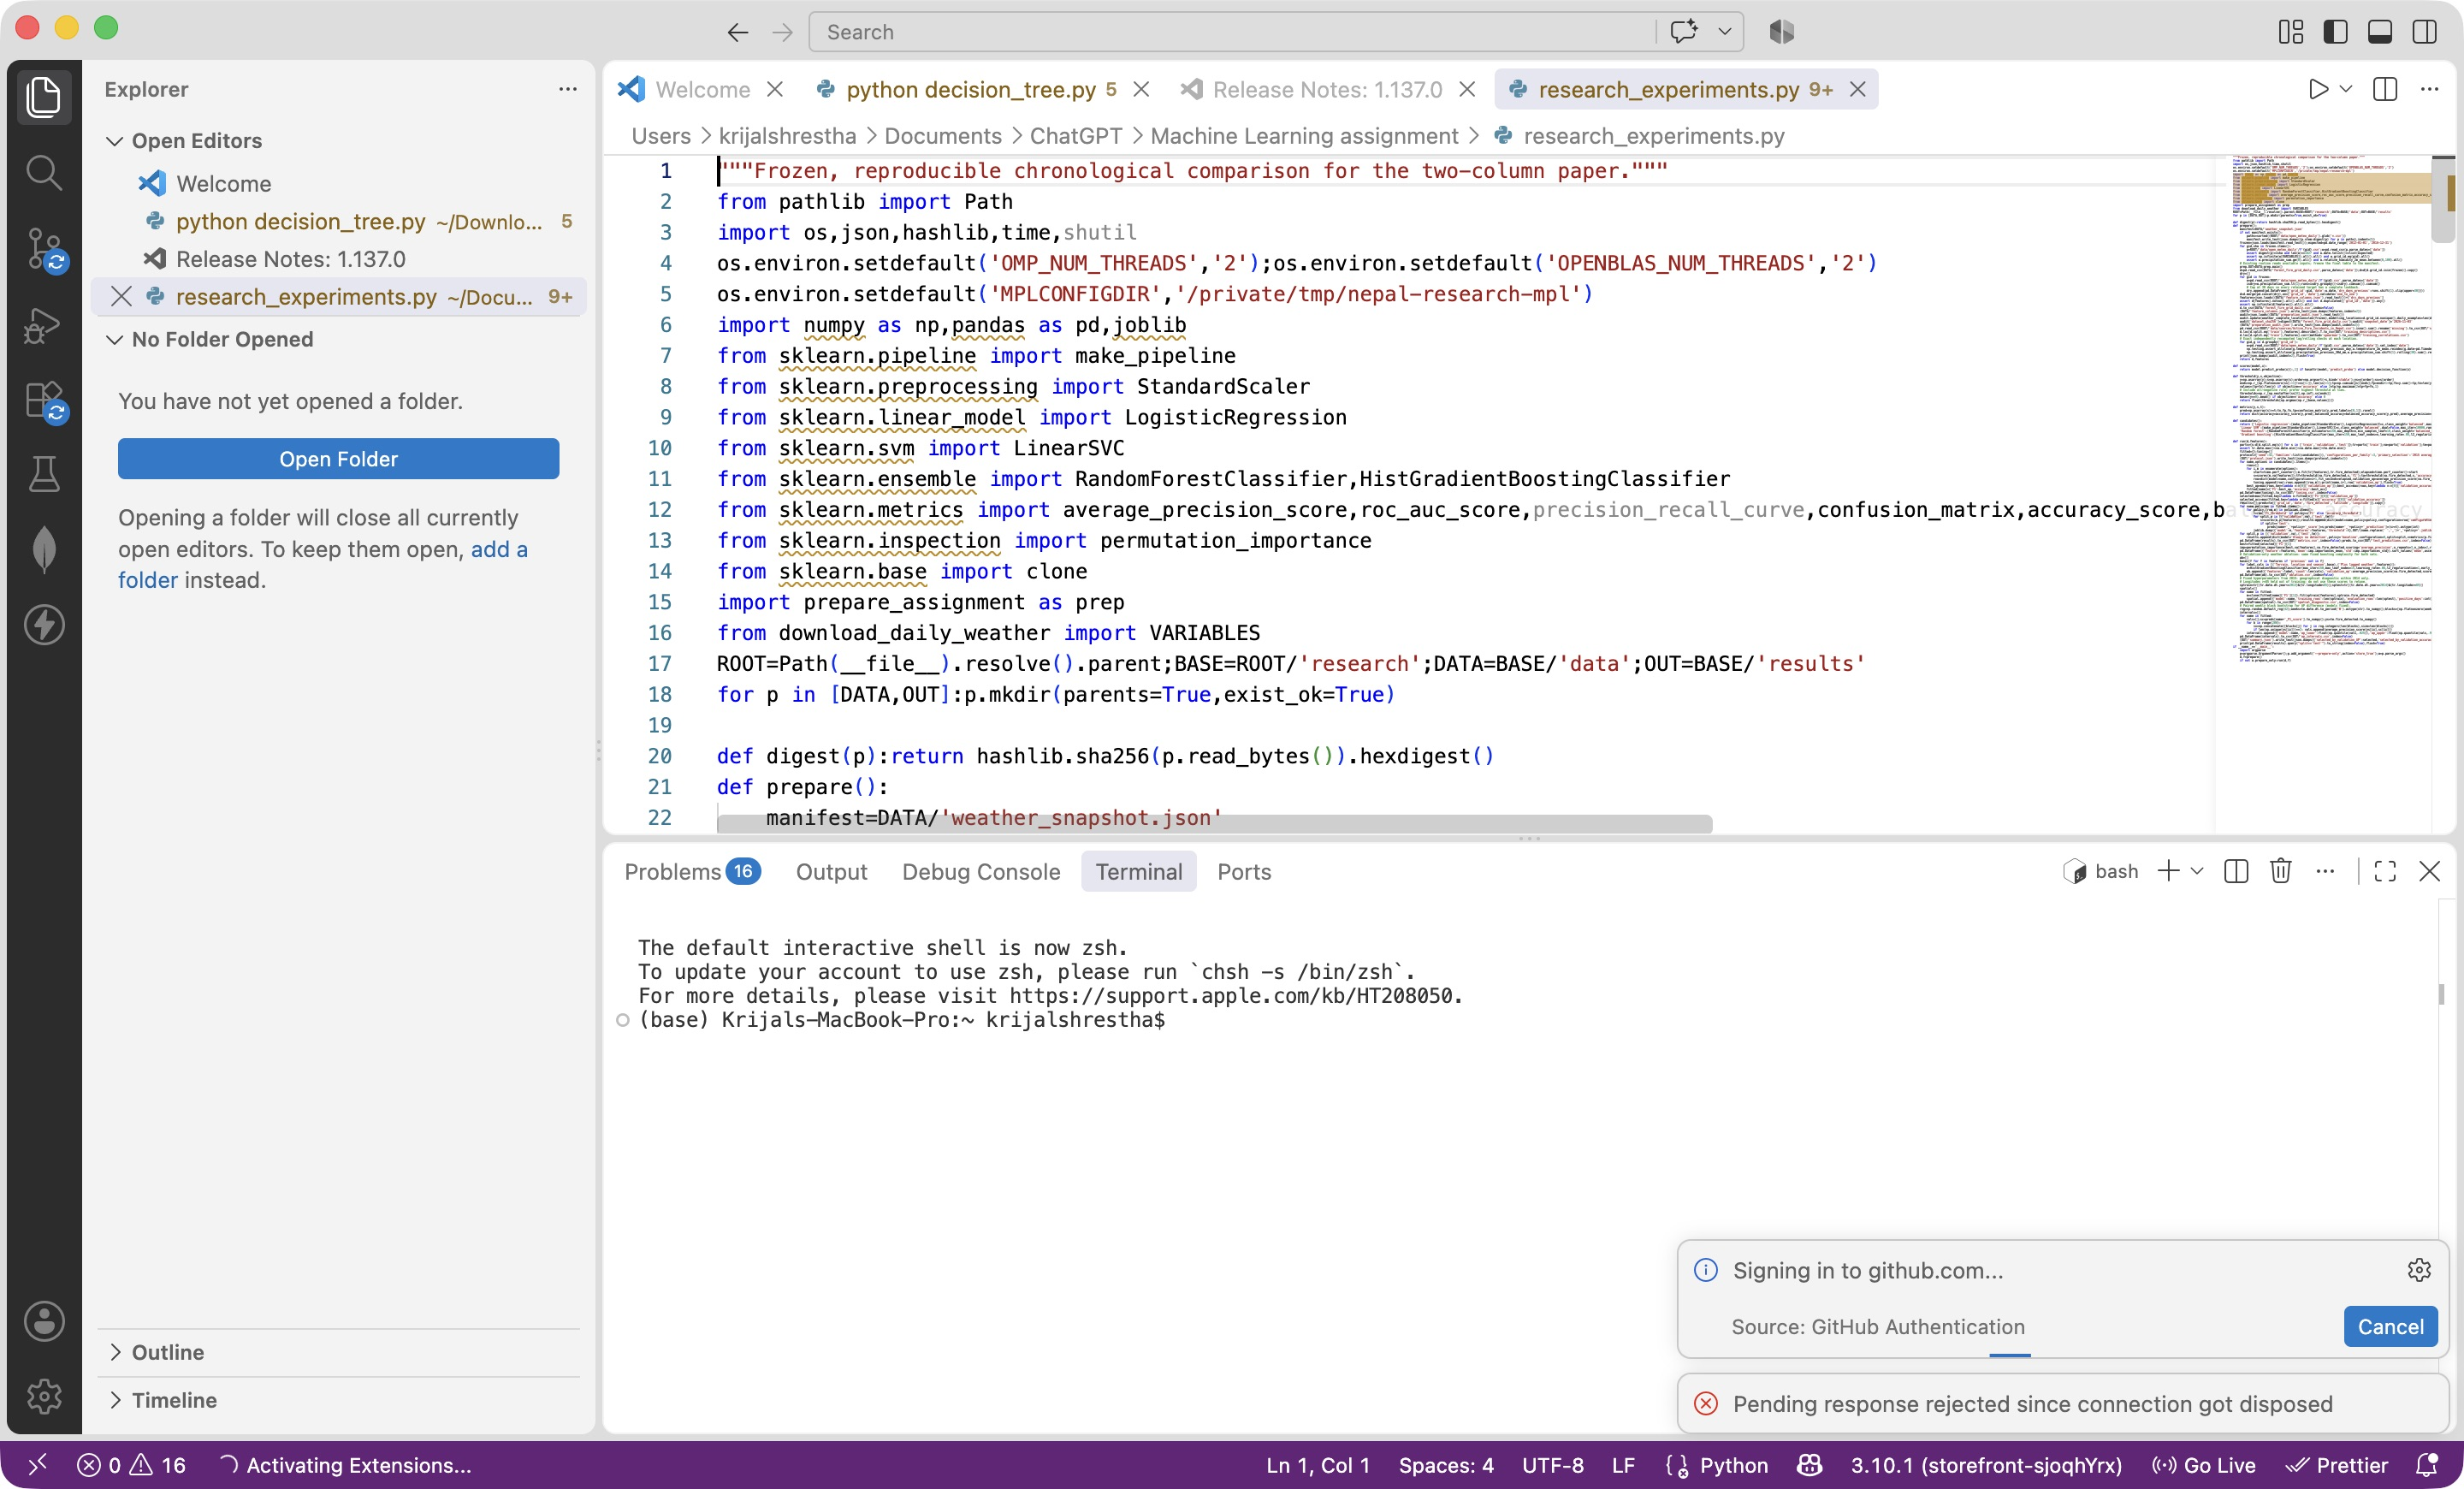
\includegraphics[width=\textwidth,trim=705 780 260 65,clip]{images/vscode_setup.png}
\caption{Project code in Visual Studio Code. The imports identify the four classifier families, scaling pipeline, evaluation metrics and data-preparation module used in the experiment.}
\label{fig:vscode}
\end{figure*}

\subsection{Weather Features and Next-Day Labels}
The one-day shift keeps the target day's weather out of the predictors. Several satellite detections in one cell-day are combined into a single positive label.
\lstinputlisting[language=Python,firstnumber=133]{code/feature_preparation.py}

\subsection{Model Fitting and Validation}
Each candidate is fitted on the training partition. Validation scores determine the model configuration and decision threshold before the later test period is evaluated.
\lstinputlisting[language=Python,firstnumber=90]{code/model_selection.py}

\end{document}
